Following the experimental process described in Section \ref{sec:sys_eval}, 120 experiments were performed 50 times each for statistical significance. This section highlights the main results from the performed experiments.

\subsection{Writing Experiments}

Figures \ref{fig:res_throughput_writing} shows the write throughput of all three pipelines defined in Section \ref{subsec:experimental_design} when writing the five different tables defined in Section \ref{subsec:dataset}. This experiment makes use of 1 \gls{CPU} core. 

Each value reported was calculated by measuring the time taken to write the table. An example consists of delta-rs on \gls{HopsFS} which took 184.12783 seconds to write 60 M rows, so dividing the rows by time the throughput obtained is 325860.566 rows/second. This result is then resampled using the bootstrapping technique, and the average, in this case 339.288 K rows/second is obtained. A 95\% confidence interval was also calculated (in this case \textpm 5.05 K rows/second), but it was not displayed in the graph as it would be hardly readable as all results are out of each other's 95\% confidence interval.

\begin{figure}
    \centering
    \begin{subfigure}[b]{\textwidth}
        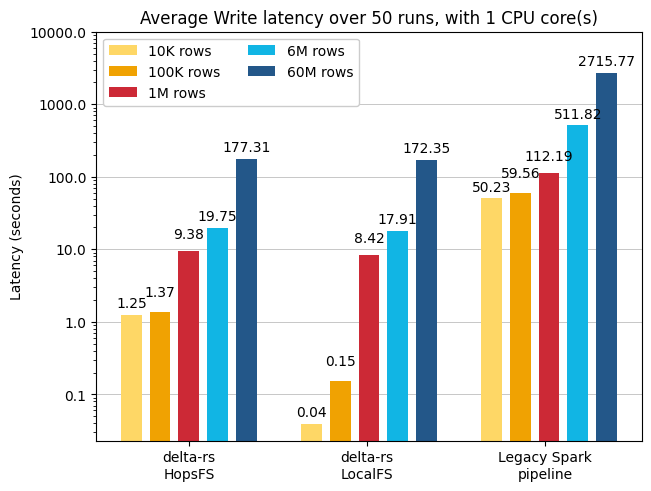
\includegraphics[width=\textwidth]{figures/5-results/write/write_time_1_core.png}
        \caption{Histogram with write latency experiment results}
        \label{fig:res_write_time}
    \end{subfigure}
    
    \begin{subfigure}[b]{\textwidth}
        \begin{tabular}{c c c c c c} 
            \toprule
            Pipeline\Tstrut\Bstrut & \thead{Number\\ of rows} & \thead{1 CPU core latency \\ (seconds)} & \thead{2 CPU cores\\ (\% decrease)} & \thead{4 CPU cores\\ (\% decrease)} & \thead{8 CPU cores\\ (\% decrease)} \\
            \midrule
            \multirow{5}{4em}{delta-rs\\ HopsFS} & 10K & 1.250881458553 & -0.92 & 2.75 & -9.33\\ 
            & 100K & 1.368281275251 & 4.40 & 2.34 & 5.54\\ 
            & 1M &   9.381529912744 & 9.23 & 10.32 & 11.52\\
            & 6M &   19.75469028131 & 17.54 & 17.87 & 20.33\\
            & 60M &  177.3070700216 & 24.39 & 30.01 & 31.22\\
            \midrule
            \multirow{5}{4em}{delta-rs\\ LocalFS} & 10K & 0.039575374951 & -21.88 & -15.53 & -11.25\\ 
            & 100K & 0.152402458205 & 10.01 & 13.54 & 10.45\\ 
            & 1M &   8.422528293415 & 14.69 & 14.68 & 14.17\\
            & 6M &   17.90634508900 & 14.74 & 18.71 & 20.24\\
            & 60M &  172.3455279090 & 24.67 & 29.57 & 30.38\\
            \midrule
            \multirow{5}{4em}{Legacy \\ Spark} & 10K & 50.22767340044 & -0.99 & -2.10 & -1.99\\ 
            & 100K & 59.56187132072 & -0.38 & 0.06 & -1.20\\ 
            & 1M &   112.1904872782 & 3.23 & 3.01 & 2.50\\
            & 6M &   511.8169330835 & 7.51 & 5.83 & 7.01\\
            & 60M &  2715.772857148 & 13.81 & 13.61 & 14.39\\
            \bottomrule
        \end{tabular}
        \caption{Table containing the write latency experiment results compared across multiple \glstext{CPU} configurations}
        \label{tbl:res_write_time_cpu_perc}
    \end{subfigure}
    \caption{Histogram (a) and Table (b) reporting the write latency experiment results also across different \glstext{CPU} configurations}
    \label{fig_tbl:res_write_time}
\end{figure}

\begin{figure}
    \centering
    \begin{subfigure}[b]{\textwidth}
        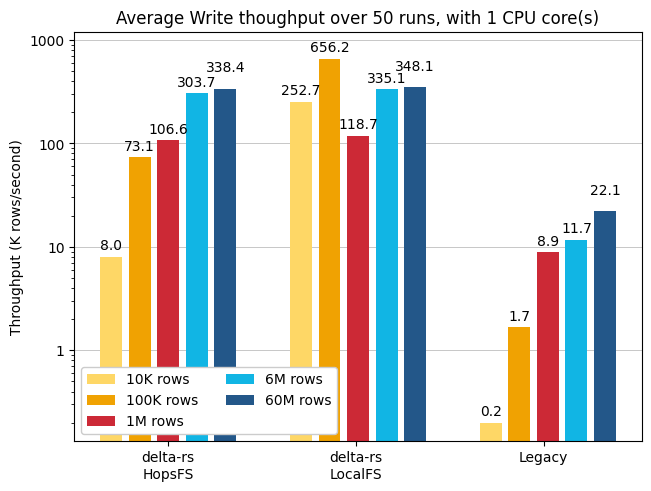
\includegraphics[width=\textwidth]{figures/5-results/write/write_throughput_1_core.png}
        \caption{Histogram with write throughput experiment results}
        \label{fig:res_write_throughput}
    \end{subfigure}
    
    \begin{subfigure}[b]{\textwidth}
        \begin{tabular}{c c c c c c} 
            \toprule
            Pipeline\Tstrut\Bstrut & \thead{Number\\ of rows} & \thead{1 CPU core throughput \\ (k rows/second)} & \thead{2 CPU cores\\ (\% increase)} & \thead{4 CPU cores\\ (\% increase)} & \thead{8 CPU cores\\ (\% increase)} \\
            \midrule
            \multirow{5}{4em}{delta-rs\\ HopsFS} & 10K & 7994.362640538 & -0.91 & 2.83 & -8.53\\ 
            & 100K & 73084.38828236 & 4.60 & 2.40 & 5.87\\ 
            & 1M &   106592.4224834 & 10.17 & 11.51 & 13.01\\
            & 6M &   303725.3388718 & 21.27 & 21.76 & 25.52\\
            & 60M &  338395.9815741 & 32.26 & 42.87 & 45.39\\
            \midrule
            \multirow{5}{4em}{delta-rs\\ LocalFS} & 10K & 252682.3817158 & -17.95 & -13.44 & -10.12\\ 
            & 100K & 656157.3952099 & 11.13 & 15.66 & 11.67\\ 
            & 1M &   118729.1945082 & 17.22 & 17.21 & 16.51\\
            & 6M &   335076.7546463 & 17.29 & 23.02 & 25.38\\
            & 60M &  348137.8410449 & 32.76 & 41.99 & 43.65\\
            \midrule
            \multirow{5}{4em}{Legacy \\ Spark} & 10K & 199.0934344156 & -0.98 & -2.06 & -1.95\\ 
            & 100K & 1678.926430325 & -0.38 & 0.06 & -1.19\\ 
            & 1M &   8913.411682753 & 3.34 & 3.10 & 2.57\\
            & 6M &   11722.94156790 & 8.12 & 6.19 & 7.54\\
            & 60M &  22093.15843262 & 16.02 & 15.76 & 16.81\\
            \bottomrule
        \end{tabular}
        \caption{Table containing the write throughput experiment results compared across multiple \glstext{CPU} configurations}
        \label{tbl:res_write_throughput_cpu_perc}
    \end{subfigure}
    \caption{Histogram (a) and Table (b) reporting the write throughput experiment results also across different \glstext{CPU} configurations}
    \label{fig_tbl:res_write_throughput}
\end{figure}

\subsection{Reading Experiments}

Figures \ref{fig:res_throughput_reading} shows the read throughput of all three pipelines defined in Section \ref{subsec:experimental_design} when writing the five different tables defined in Section \ref{subsec:dataset}. This experiment makes use of 1 \gls{CPU} core. 

Each value reported was calculated by measuring the time taken to read the table. An example consists of delta-rs on \gls{HopsFS} which took 0.0378069 seconds to read 60 M rows, so dividing the rows by time the throughput obtained is 1587.0114 M rows/second. This result is then resampled using the bootstrapping technique, and the average, in this case 1929.861 M rows/second is obtained. A 95\% confidence interval was also calculated (in this case \textpm 102.7 M rows/second), but it was not displayed in the graph as it would be hardly readable as all results are out of each other's 95\% confidence interval.

\begin{figure}
    \centering
    \begin{subfigure}[b]{\textwidth}
        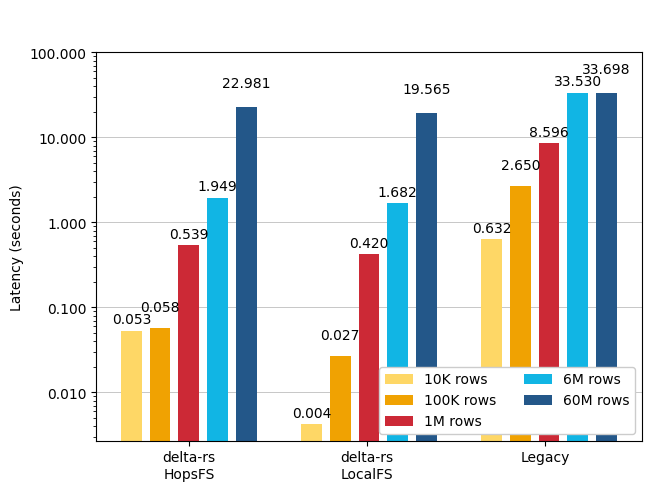
\includegraphics[width=\textwidth]{figures/5-results/read/read_time_1_core.png}
        \caption{Histogram with read latency experiment results}
        \label{fig:res_read_time}
    \end{subfigure}
    
    \begin{subfigure}[b]{\textwidth}
        \begin{tabular}{c c c c c c} 
            \toprule
            Pipeline\Tstrut\Bstrut & \thead{Number\\ of rows} & \thead{1 CPU core latency \\ (seconds)} & \thead{2 CPU cores\\ (\% decrease)} & \thead{4 CPU cores\\ (\% decrease)} & \thead{8 CPU cores\\ (\% decrease)} \\
            \midrule
            \multirow{5}{4em}{delta-rs\\ HopsFS} & 10K & 0.053427784961 & 22.65 & 18.84 & 18.95\\ 
            & 100K & 0.057573573334 & 1.15 & 3.76 & 5.19\\ 
            & 1M & 0.538551778791 & 56.53 & 65.00 & 67.71\\
            & 6M & 1.948992908833 & 53.40 & 72.74 & 74.48\\
            & 60M & 22.98065653875 & 50.34 & 75.72 & 87.20\\
            \midrule
            \multirow{5}{4em}{delta-rs\\ LocalFS} & 10K & 0.004193598319 & 31.48 & 35.91 & 29.66\\ 
            & 100K & 0.026966840860 & 51.54 & 65.76 & 64.84\\ 
            & 1M &   0.420096789910 & 52.45 & 78.64 & 89.75\\
            & 6M &   1.682239274377 & 55.56 & 77.99 & 89.57\\
            & 60M &  19.56547400704 & 51.72 & 75.41 & 88.32\\
            \midrule
            \multirow{5}{4em}{Legacy \\ Spark} & 10K & 0.631598152258 & 1.06 & -0.67 & 0.67\\ 
            & 100K & 2.650107346201 & -0.50 & 0.39 & -0.46\\ 
            & 1M &   8.596367535570 & -0.24 & -1.81 & 2.89\\
            & 6M &   33.52964549822 & 0.46 & 0.23 & 0.30\\
            & 60M &  33.69772492026 & 0.16 & 0.13 & 1.64\\
            \bottomrule
        \end{tabular}
        \caption{Table containing the read latency experiment results compared across multiple \glstext{CPU} configurations}
        \label{tbl:res_read_time_cpu_perc}
    \end{subfigure}
    \caption{Histogram (a) and Table (b) reporting the read latency experiment results also across different \glstext{CPU} configurations}
    \label{fig_tbl:res_read_time}
\end{figure}

\begin{figure}
    \centering
    \begin{subfigure}[b]{\textwidth}
        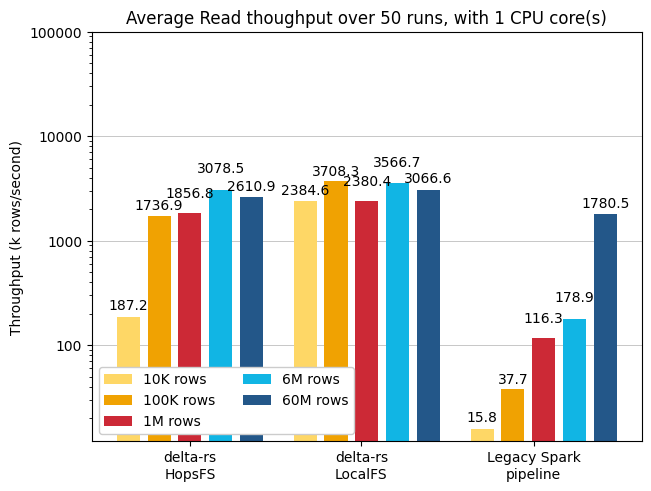
\includegraphics[width=\textwidth]{figures/5-results/read/read_throughput_1_core.png}
        \caption{Histogram with read throughput experiment results}
        \label{fig:res_read_throughput}
    \end{subfigure}
    
    \begin{subfigure}[b]{\textwidth}
        \begin{tabular}{c c c c c c} 
            \toprule
            Pipeline\Tstrut\Bstrut & \thead{Number\\ of rows} & \thead{1 CPU core throughput \\ (k rows/second)} & \thead{2 CPU cores\\ (\% increase)} & \thead{4 CPU cores\\ (\% increase)} & \thead{8 CPU cores\\ (\% increase)} \\
            \midrule
            \multirow{5}{4em}{delta-rs\\ HopsFS} & 10K & 187168.5305156 & 29.28 & 23.21 & 23.38\\ 
            & 100K & 1736907.998044 & 1.17 & 3.90 & 5.48\\ 
            & 1M &   1856831.672237 & 130.02 & 185.74 & 209.69\\
            & 6M &   3078512.996536 & 114.57 & 266.87 & 291.92\\
            & 60M &  2610891.464254 & 101.35 & 311.83 & 681.03\\
            \midrule
            \multirow{5}{4em}{delta-rs\\ LocalFS} & 10K & 2384586.991466 & 45.94 & 56.04 & 42.18\\ 
            & 100K & 3708257.875522 & 106.37 & 192.07 & 184.38\\ 
            & 1M &   2380403.811732 & 110.28 & 368.24 & 875.15\\
            & 6M &   3566674.545879 & 125.01 & 354.40 & 858.64\\
            & 60M &  3066626.445053 & 107.11 & 306.75 & 756.07\\
            \midrule
            \multirow{5}{4em}{Legacy \\ Spark} & 10K & 15832.85189203 & 1.07 & -0.67 & 0.67\\ 
            & 100K & 37734.32051472 & -0.50 & 0.39 & -0.45\\ 
            & 1M &   116328.2044261 & -0.24 & -1.78 & 2.98\\
            & 6M &   178946.1209876 & 0.46 & 0.23 & 0.30\\
            & 60M &  1780535.633843 & 0.16 & 0.13 & 1.67\\
            \bottomrule
        \end{tabular}
        \caption{Table containing the read throughput experiment results compared across multiple \glstext{CPU} configurations}
        \label{tbl:res_read_throughput_cpu_perc}
    \end{subfigure}
    \caption{Histogram (a) and Table (b) reporting the read throughput experiment results also across different \glstext{CPU} configurations}
    \label{fig_tbl:res_read_throughput}
\end{figure}

\subsection{Experiments with more \glsfmtshort{CPU} cores}

Experiments reading and writing tables from the TPC-H benchmark in the three different pipelines defined in Section \ref{subsec:experimental_design} were repeated with increasingly more \gls{CPU} cores. The Tables \ref{tbl:cpu_percent_diff_write} and \ref{tbl:cpu_percent_diff_read} display the percentage increase between the first and the increased \gls{CPU} cores experiment. For example the delta-rs \gls{HopsFS} pipeline throughput when writing a 60M rows table is 339.288979358 k rows/second, when using 1 \gls{CPU} core. During the experiment when it was using 8 \gls{CPU} cores the throughput was 494.7344718446817 k rows/second. Thus the performance increase of the throughput as a percentage is 45.82 \% (calculated as the rate between the increase and the 1 \gls{CPU} experiment multiplied by 100). Note that in some cases the performance increase is negative, meaning that the throughput decreased even if computational resources were increased.

\subsection{Writing using legacy Spark pipeline -- Time breakdown}

During the writing experiment performed using the legacy Spark pipeline the contribution of different part of the process were measured: namely the upload time and materialization time, dichotomy explained in Section \todo[inline]{Ref here time breakdown expl.}. This served to verify how different part of the legacy pipeline scaled with table sizes, and if Spark was in fact the bottleneck of the architecture.

\begin{figure}
    \centering
    \begin{subfigure}[b]{\textwidth}
        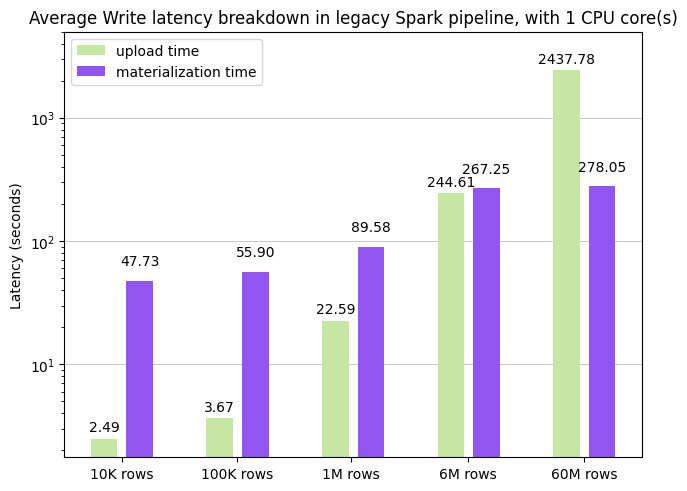
\includegraphics[width=\textwidth]{figures/5-results/hudi_virtualiz_1_core.png}
        \caption{Histogram displaying the contributions to the write latency of the upload and materialization steps in the legacy Spark pipeline}
        \label{fig:hudi_virtualiz_breakdown}
    \end{subfigure}
    
    \begin{subfigure}[b]{\textwidth}
        \begin{tabular}{c c c c c c c c c} 
            \toprule
            \multirow{2}{*}{\thead{Number\\ of rows}} & \multicolumn{2}{c}{\thead{1 CPU core\\ latency (seconds)}} & \multicolumn{2}{c}{\thead{2 CPU cores\\ (\% decrease)}} & \multicolumn{2}{c}{\thead{4 CPU cores\\ (\% decrease)}} & \multicolumn{2}{c}{\thead{8 CPU cores\\ (\% decrease)}}\\
            & upl. & mat. & upl. & mat. & upl. & mat. & upl. & mat.\\
            \midrule
            10K &  2.48653 & 47.726 & 3.99 & -1.27 & 4.10 & -2.47 & 4.22 & -2.35\\
            100K & 3.66844 & 55.900 & 6.37 & -0.78 & 5.55 & -0.27 & 6.25 & -1.69\\
            1M   & 22.5934 & 89.575 & 17.52 & -0.39 & 14.89 & -0.01 & 16.51 & -1.05\\
            6M   & 244.612 & 267.24 & 15.83 & -0.10 & 13.46 & -1.15 & 15.10 & -0.38\\
            60M &  2437.78 & 278.05 & 15.33 & 0.39 & 15.15 & 0.16 & 15.94 & 0.82\\
            \bottomrule
        \end{tabular}
        \caption{Table showing the contributions to the write latency of the upload and materialization steps in the legacy Spark pipeline and it change at different \glstext{CPU} configurations}
        \label{tbl:hudi_virtualiz_breakdown_cpu_perc}
    \end{subfigure}
    \caption{Histogram (a) and Table (b) reporting the contributions to the write latency of the upload and materialization steps in the legacy Spark pipeline and it change at different \glstext{CPU} configurations}
    \label{fig_tbl:hudi_virtualiz_breakdown}
\end{figure}

\subsection{In-memory resources usage}
\label{subsec:resources_usage}

The experimental environment resources defined in Section \ref{subsec:exp_env} were adjusted according to the computational needs. In particular, write operations were demanding on the available \gls{RAM} resources, requiring up to 24 GBs to operate with the larger tables (6M and 60M rows). The system was adjusted to allocate 32768 MB of \gls{RAM}, so it could avoid slowing down operations.